\documentclass[10pt]{article}
\usepackage{icmlko}

\icmlmeta{IP 파운데이션 월드모델}{103}{맞출 수 없는 축}{고유로 넣으면 정렬 재료를 밀어내고 공통으로 올리면 정렬이 안 된다 --- 새 축이 열두 번 $\pm$0.01에 머문 이유가 구조에 있었다}

\begin{document}

\twocolumn[
\icmlheader

\begin{abstract}
노트 102가 기제를 밝혔다 --- 고유 축을 넣으면 프로크루스테스가 쓰는 공통 축
적재가 밀려난다. 밀어냄은 공통 블록이 \textbf{셋뿐}이라 생기므로, 아홉 도메인이
공유하는 설명문 축을 \textbf{공통 슬롯으로 올리면} 밀어내는 대신 정렬 재료가
늘어야 한다. \textbf{구조는 정확히 그렇게 됐다} --- 공통 블록 적재 몫이 고유로
넣을 때 0.677$\to$0.538로 줄던 것이 공통으로 올리면 \textbf{0.677$\to$0.702로
는다.} 쌍당 공통 축도 2.64에서 3.40으로 늘어 노트 37의 제약($c\!<\!k$면 회전
과소결정)이 풀린다. \textbf{그런데 성적은 내린다} --- 고유 $k{=}3$ 이
$+$0.0127인데 공통 $k{=}2$ 는 $+$0.0025, $k{=}3$ 은 $-$0.0148, $k{=}4$ 는
$-$0.0233이다. 부호 탓인가 --- emb0 과 라벨의 상관이 애니 $+$0.229, 모바일
$-$0.229로 갈린다. 전체 자료로 \emph{반칙해서} 부호를 맞춰도 $+$0.0005다.
\textbf{부호가 아니다.} 잔차를 쟀더니 답이 나왔다 --- 원래 공통 축 셋의 정렬
상대 잔차가 0.592인데 \textbf{emb0 자신은 1.676}이다. \textbf{1을 넘는다는 것은
회전으로 맞추는 것이 안 맞추는 것보다 나쁘다는 뜻}이다. 게다가 그 축을 공통에
넣으면 \emph{원래 셋의} 잔차까지 0.592에서 0.624로 5.4\% 나빠진다.
\textbf{설명문 축은 도메인을 건너 측정 불변이 아니다}(Meredith 1993). 여기서
구조적 막다른 골목이 확인된다 --- \textbf{고유로 넣으면 밀어내고, 공통으로
올리면 안 맞는다.} 노트 84 이후 열두 개 새 축이 전부 $\pm$0.01에 머문 것은
축을 잘못 골라서가 아니라 \textbf{직교 프로크루스테스가 새 축을 받을 자리가
없어서}였다.
\end{abstract}
]

\begin{figure*}[t]
\centering
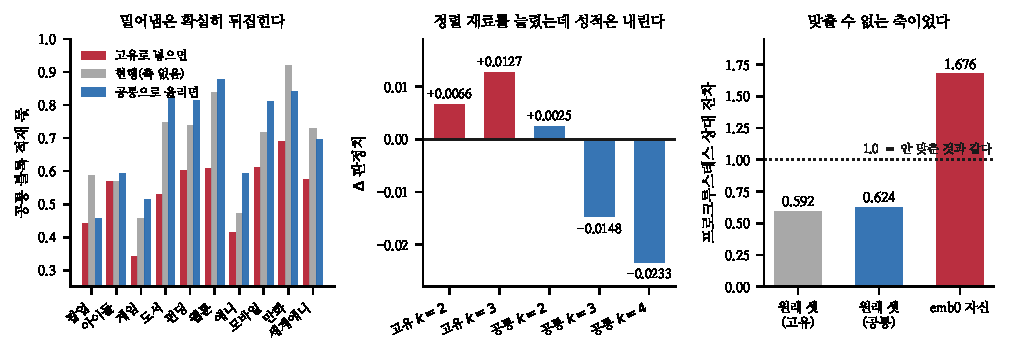
\includegraphics[width=\textwidth]{figs/un.pdf}
\caption{왼쪽 --- 밀어냄은 확실히 뒤집힌다. 가운데 --- 그래도 성적은 내린다.
오른쪽 --- 맞출 수 없는 축이었다.}
\end{figure*}

\section{구조는 의도대로 됐다}

지금 공통 축은 셋이다 --- 타깃 폭 · 굿즈 규모 · 매장 노출. 쌍마다 둘만
겹치는 경우도 많아 평균 \textbf{2.64}다. 설명문 축은 아홉 도메인이 가지므로
공통으로 올릴 수 있다.

\begin{table}[t]
\centering\tsize
\caption{공통 블록이 상위 성분 적재에서 차지하는 몫.}
\begin{tabular}{lrrr}
\toprule
& 현행 & 고유로 & \textbf{공통으로} \\
\midrule
웹툰 & 0.837 & 0.609 & \textbf{0.877} \\
만화 & 0.920 & 0.689 & 0.840 \\
모바일 & 0.716 & 0.610 & \textbf{0.812} \\
도서 & 0.747 & 0.531 & \textbf{0.822} \\
펀딩 & 0.738 & 0.601 & \textbf{0.814} \\
애니 & 0.472 & 0.414 & \textbf{0.594} \\
게임 & 0.458 & 0.341 & \textbf{0.513} \\
팝업 & 0.587 & 0.441 & 0.457 \\
\midrule
\textbf{평균} & 0.677 & \textbf{0.538} & \textbf{0.702} \\
\midrule
쌍당 공통 축 & 2.64 & 2.64 & \textbf{3.40} \\
\bottomrule
\end{tabular}
\end{table}

\claimx{노트 102의 밀어냄이 \textbf{정확히 뒤집힌다.} 고유로 넣으면 공통 블록
몫이 0.677에서 0.538로 주는데, 공통으로 올리면 0.702로 는다. 쌍당 정렬 재료도
2.64에서 3.40으로 늘어 $k{=}3$ 이 과소결정이 아니게 된다.}{팝업만 예외다
(0.587$\to$0.457) --- 팝업은 설명문 덮개율이 91\%라 결측 표시자가 고유 축으로
하나 더 붙기 때문이다.}

\section{그런데 성적은 내린다}

\begin{table}[t]
\centering\tsize
\caption{설명문 축 하나. 아홉 도메인.}
\begin{tabular}{lrrr}
\toprule
& $\rho$ & $\Delta$ & 팝업 \\
\midrule
현행(축 없음) & $+$0.4038 & --- & $+$0.4501 \\
고유 · $k{=}2$ & $+$0.4104 & $+$0.0066 & $+$0.4537 \\
\textbf{고유 · $k{=}3$} & \textbf{$+$0.4165} & \textbf{$+$0.0127} & $+$0.4578 \\
공통 · $k{=}2$ & $+$0.4063 & $+$0.0025 & $+$0.4568 \\
공통 · $k{=}3$ & $+$0.3890 & $-$0.0148 & $+$0.4263 \\
공통 · $k{=}4$ & $+$0.3805 & $-$0.0233 & $+$0.4273 \\
\midrule
표지 · 고유 · $k{=}3$ & $+$0.4002 & $-$0.0036 & $+$0.4599 \\
표지 · 공통 · $k{=}3$ & $+$0.3906 & $-$0.0132 & $+$0.4526 \\
둘 다 · 공통 · $k{=}3$ & $+$0.3723 & $-$0.0315 & $+$0.4269 \\
\bottomrule
\end{tabular}
\end{table}

\claimx{정렬 재료를 늘렸는데 성적이 내린다. 그리고 \textbf{공통 축을 늘릴수록,
성분을 늘릴수록 더 내린다} --- 공통 $k{=}4$ 가 $-$0.0233, 설명문과 표지를 둘 다
공통으로 올리면 $-$0.0315다.}{$k$ 를 올린 것과 공통으로 올린 것이 섞여 있다.
다만 $k{=}2$ 로 고정해도 공통($+$0.0025)이 고유($+$0.0066)보다 낮다.}

\section{부호 탓이 아니다}

공통 축이 되려면 도메인을 건너 같은 것을 재야 한다. 설명문 축은 라벨과의
부호부터 갈린다.

\begin{table}[t]
\centering\tsize
\caption{emb0 과 그 도메인 라벨의 상관.}
\begin{tabular}{lrlr}
\toprule
애니 & $+$0.229 & 게임 & $+$0.116 \\
모바일 & \textbf{$-$0.229} & 팝업 & $+$0.049 \\
세계애니 & $+$0.191 & 펀딩 & $+$0.046 \\
도서 & \textbf{$-$0.094} & 만화 & $+$0.035 \\
웹툰 & $+$0.008 & & \\
\bottomrule
\end{tabular}
\end{table}

부호가 음수인 도메인에서 축을 뒤집어 봤다 --- \textbf{전체 자료로 반칙해서}
맞춘 것이라 낙관적 상한이다.

\begin{table}[t]
\centering\tsize
\caption{부호를 맞추면.}
\begin{tabular}{lrr}
\toprule
& $\rho$ & $\Delta$ \\
\midrule
공통 · 부호 그대로 · $k{=}2$ & $+$0.4063 & $+$0.0025 \\
공통 · \textbf{전체 부호 맞춤} · $k{=}2$ & $+$0.4043 & $+$0.0005 \\
공통 · 부호 그대로 · $k{=}3$ & $+$0.3890 & $-$0.0148 \\
공통 · \textbf{전체 부호 맞춤} · $k{=}3$ & $+$0.3911 & $-$0.0127 \\
\midrule
보정 표본 50\%로 정직하게 & $+$0.4082 & $+$0.0044 \\
\bottomrule
\end{tabular}
\end{table}

\claimx{부호가 원인이 아니다. \textbf{반칙해서 맞춰도} $+$0.0005다. 노트 69의
방향 문제와는 다른 종류의 불일치다.}{보정 표본 50\%로 정한 부호가 $+$0.0044로
가장 낫다. 반칙보다 나은 것이 이상한데, 부호가 흔들리는 도메인에서 표본 잡음이
우연히 나은 쪽을 골랐을 수 있다 --- 다섯 씨앗 평균이라 우연으로 보인다.}

\section{맞출 수 없는 축이었다}

프로크루스테스가 실제로 얼마나 맞추는지 쟀다 --- 회전 뒤 적재 차이를 대상
적재 크기로 나눈 \textbf{상대 잔차}. 1을 넘으면 맞추는 것이 안 맞추는 것보다
나쁘다는 뜻이다.

\begin{table}[t]
\centering\tsize
\caption{상대 잔차. 쌍 88개.}
\begin{tabular}{lr}
\toprule
원래 공통 축 셋 (emb0 은 고유) & 0.592 \\
원래 공통 축 셋 (emb0 을 공통에 넣고) & 0.624 \quad($+$5.4\%) \\
\textbf{emb0 자신} & \textbf{1.676} \\
\bottomrule
\end{tabular}
\end{table}

\claimx{\textbf{설명문 축은 도메인을 건너 정렬되지 않는다.} 상대 잔차가 1.676
--- 하나의 직교 회전으로 아홉 도메인의 emb0 적재를 맞추는 것이 아예 안 맞추는
것보다 나쁘다. 게다가 그 축을 공통에 넣으면 \emph{맞출 수 있는} 셋의 잔차까지
5.4\% 나빠진다.}{잔차는 적재 공간의 거리이지 전이 성적이 아니다. 다만 방향과
크기가 성적 표와 일치한다.}

\begin{table}[t]
\centering\tsize
\caption{공통 축 \emph{수}를 셋으로 고정하고 하나를 emb0 으로 바꾸면.}
\begin{tabular}{lr}
\toprule
& $\Delta$ \\
\midrule
타깃 폭 $\to$ emb0 & $-$0.1306 \\
굿즈 규모 $\to$ emb0 & $-$0.0225 \\
매장 노출 $\to$ emb0 & $-$0.0158 \\
\midrule
\textbf{그대로 두고 emb0 은 고유} & \textbf{$+$0.0066} \\
\bottomrule
\end{tabular}
\end{table}

\section{구조적 막다른 골목}

\begin{quote}\fontsize{9.5}{11.5}\selectfont
\textbf{고유로 넣으면 밀어내고(노트 102), 공통으로 올리면 안 맞는다(이 노트).}
노트 84 이후 열두 개 새 축이 전부 $\pm$0.01에 머문 것은 축을 잘못 골라서가
아니었다 --- \textbf{직교 프로크루스테스가 새 축을 받을 자리가 없다.} 정렬은
측정 불변을 요구하는데(Meredith 1993) 도메인마다 다른 플랫폼에서 긁은 축은
그 조건을 못 채운다.
\end{quote}

\claimx{남은 길은 \textbf{정렬을 바꾸는 것}이다. 하나의 직교 회전 대신 쌍마다
\emph{배우는} 사상이면 측정 불변이 필요 없다.}{노트 93이 정렬 없는 직접 전이를
시도해 $-$0.032였고, 노트 85--88의 공유 인코더도 졌다. \textbf{``배우는 사상''도
같은 이유로 질 수 있다} --- 팝업 표본 75건으로는 쌍별 사상을 학습할 자료가 없다.}

\section{한계}

\begin{itemize}[leftmargin=1.1em,itemsep=0.15em]
\item \textbf{채택할 것이 없다.} 이 노트의 모든 공통 설정이 고유 설정보다
      나쁘다.
\item 잔차와 성적을 회귀로 잇지 않았다. 방향만 일치한다.
\item 공통으로 올린 축이 emb0 하나와 imgpc0 하나뿐이다. 다른 축은 정렬될
      수도 있다.
\item 부호 보정에서 50\%가 반칙보다 나은 것을 설명 못 한다.
\item 노트 102가 남긴 시간 분할 판정(노트 77)은 이번에도 안 했다.
\end{itemize}

\section{다음}

\begin{enumerate}[leftmargin=1.3em,itemsep=0.15em]
\item \textbf{정렬을 배우게 한다} --- 직교 회전 대신 쌍마다 최소제곱 선형
      사상(비직교, 축소계수 포함). 직교 제약만 푸는 것이라 표본이 적어도
      추정 가능하다. 이것이 노트 93 · 88의 실패와 다른 점이다.
\item \textbf{어떤 축이 정렬되는지 미리 잰다} --- 잔차 1.676을 \emph{긁기 전에}
      알 수 있으면 노트 101의 지침을 잔차로 다시 세울 수 있다. 라벨 상관이
      아니라 \textbf{정렬 가능성}이 기준이어야 한다.
\item 공통 축을 늘리는 다른 길 --- 지금 셋은 전부 사람이 매긴 것이다.
      도메인 넷 이상이 같은 플랫폼에서 긁은 축이 있으면 정렬될 수 있다.
\item 시간 분할 판정(노트 77). 반쪽 검정이 표본을 반으로 줄이는 문제를 피한다.
\end{enumerate}

\vspace{0.6em}
\hrule height 0.3pt
\vspace{0.5em}
{\footnotesize
\textbf{참고문헌}\\[0.3em]
Meredith, W. (1993). Measurement invariance, factor analysis and factorial
invariance. \emph{Psychometrika}, 58(4), 525--543.\\[0.15em]
Schoenemann, P. H. (1966). A generalized solution of the orthogonal Procrustes
problem. \emph{Psychometrika}, 31(1), 1--10.\\[0.15em]
Ben-David, S. et al. (2010). A theory of learning from different domains.
\emph{Machine Learning}, 79(1--2), 151--175.\\[0.15em]
Gower, J. C., Dijksterhuis, G. B. (2004). \emph{Procrustes Problems}.
Oxford University Press.\\[0.15em]
Cawley, G. C., Talbot, N. L. C. (2010). On over-fitting in model selection and
subsequent selection bias in performance evaluation. \emph{JMLR}, 11, 2079--2107.
}

\end{document}
